%%%%%%%%%%%%%%%%%%%%%%%%%%%%%%%%%%%%%%%%%%%%%%%%%%%%%%%%%%%%%%%%%%%%%%%%%%%%%% 
\newpage
\section {SINDRUM-II momentum scale }

In \cite{sindrum_ii:Bertl2006}, the momentum scale has been calibrated using
the edge of the Michel spectrum from muon decays $\mu^+ \rightarrow e^+ \nu \bar{\nu}$
at rest. The calibration has been performed with the magnetic field reduced to about 50\%
of the nominal value. The reconstructed positron momentum distribution is shown
in Figure \ref{fig:sindrum_ii_fig_08_fit}.

\begin{figure}
\begin{tikzpicture}
  \node[anchor=south west,inner sep=0] at (0,0.) {
    % \node[shift={(0 cm,0.cm)},inner sep=0,rotate={90}] at (0,0) {}
    \makebox[\textwidth][c] {
      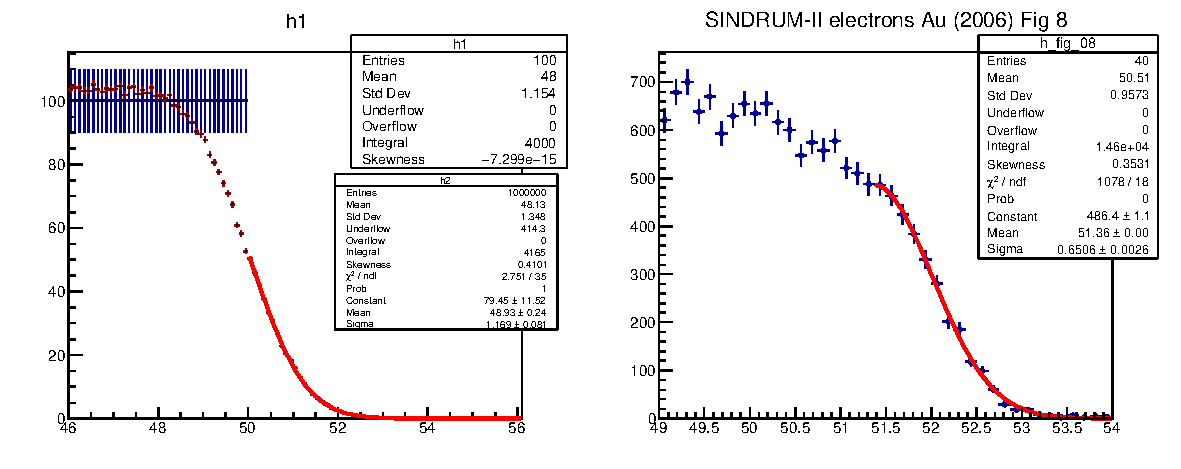
\includegraphics[width=0.99\textwidth]{figures/pdf/sindrum_ii_fig_08_fit}
    }
  };
  % \node [text width=6cm, scale=0.8] at (4.5,6.4) {mu2e-18894 by Kevin Lynch and Jim Popp};
\end{tikzpicture}
% \captionof{figure} {
\caption{
  \label{fig:sindrum_ii_fig_08_fit}
  Reconstructed momentum spectrum of positrons from $\mu^+ \rightarrow e^+ \nu \bar{\nu}$
  decays used in \cite{sindrum_ii:Bertl2006} for detector momentum calibration.
}
\end{figure}

Although radiative corrections modify the positron spectrum, as shown in Figure \ref{fig:mu2e_5645_fig_001_mue3_decay} their impact on the edge of the Michel spectrum
is fairly small, and the reconstructed position and shape of the edge depend primarily
on the energy losses and the momentum resolution.

\begin{tikzpicture}
  \node[anchor=south west,inner sep=0] at (0,0.) {
    % \node[shift={(0 cm,0.cm)},inner sep=0,rotate={90}] at (0,0) {}
    \makebox[\textwidth][c] {
      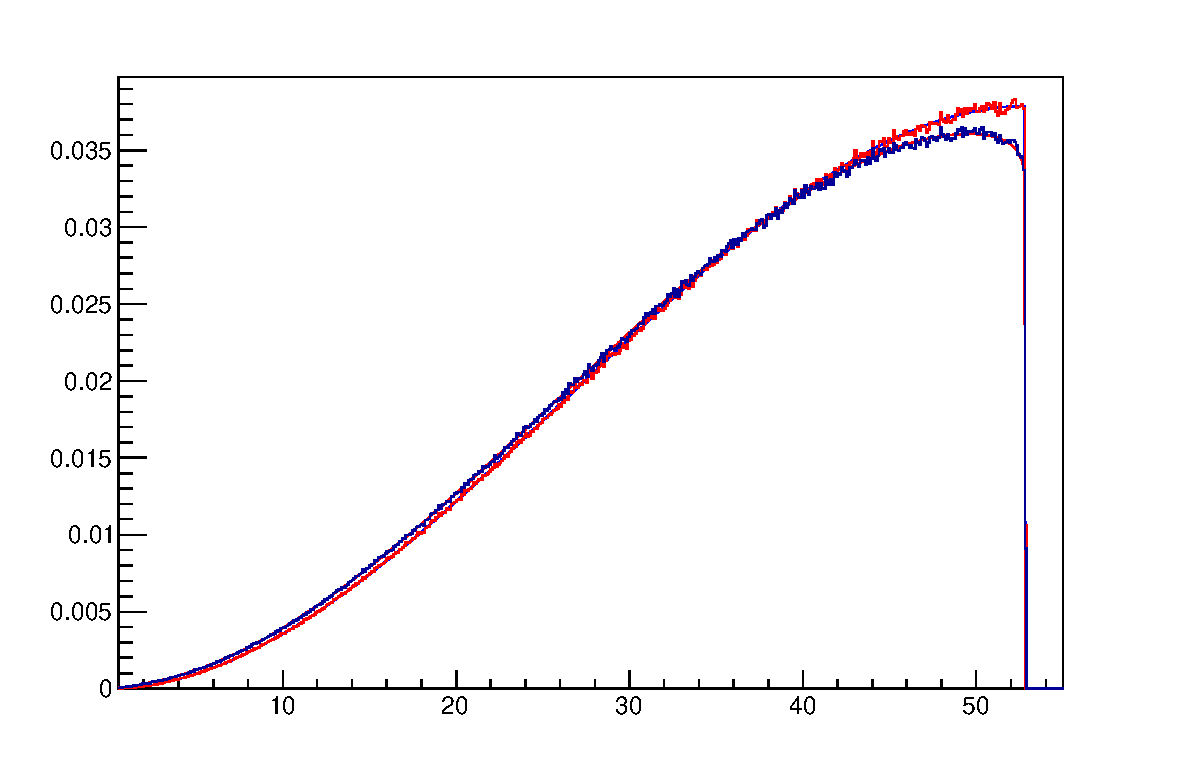
\includegraphics[width=0.99\textwidth]{figures/pdf/mu2e_5645_fig_001_mue3_decay}
    }
  };
  % \node [text width=6cm, scale=0.8] at (4.5,6.4) {mu2e-18894 by Kevin Lynch and Jim Popp};
\end{tikzpicture}
\captionof{figure} {
  \label{fig:mu2e_5645_fig_001_mue3_decay}
  Monte Carlo momentum spectrum of positrons from the $\mu^+ \rightarrow e^+ \nu \bar{\nu}$
  decay. Red: leading order, Blue: with radiative corrections taken into account.
}
\vspace{0.1in}

We expect the positron momentum referred to in the paper
to be the momentum in the first reconstructed point on the trajectory. As such, the
reconstructed Michel edge should be affected by the energy losses in front of the
tracker, their fluctuations, as well as the momentum resolution of the tracker.
According to \cite{sindrum_ii:Bertl2006}, the energy losses in front of the tracker
are due to losses in the Au target (75 mg/cm$^2$) and the wall of the
vacuum chamber (324 mg/cm$^2$), main components of which are aluminum and carbon fiber.

To validate our understanding of the SINDRUM-II momentum calibration,
we simulate energy losses of positrons with initial momenta distributed uniformly
in the range [45,52.8] MeV/c in a structure consisting of the two layers described
above. The initial momentum distribution is shown
in Figure ~\ref{fig:sindrum_ii_michel_calibration} in red,
the positron momentum distribution on exit from the vacuum chamber wall is shown in blue.
Comparison of the two distributions shows that for a $\sim$ 50 MeV electron, the most probable
energy loss in front of the SINDRUM-II tracker is about 0.6 MeV

Shaded is the positron momentum distribution on exit convolved with
a Gaussian with $\sigma = 0.55$ MeV/c corresponding to the SINDRUM-II
momentum resolution of 1.3 MeV/c FWHM \cite{sindrum_ii:Kaulard1997_Thesis}.
The shaded distribution in Figure ~\ref{fig:sindrum_ii_michel_calibration}
double counts the fluctuations of energy losses, however the impact of double
counting is small and momentum edge smearing is dominated by the momentum
resolution of the tracker.

The fit of the high-momentum part of the smeared edge with the Gaussian returns
$\sigma = 0.63 \pm 0.03$ MeV/c, in good agreement with $\sigma = 0.65 \pm 0.06$ MeV/c
returned by the fit of the SINDRUM-II spectrum in Figure ~\ref{fig:sindrum_ii_fig_08_fit}.

\begin{figure} 
\begin{tikzpicture}
  \node[anchor=south west,inner sep=0] at (0,0.) {
    % \node[shift={(0 cm,0.cm)},inner sep=0,rotate={90}] at (0,0) {}
    \makebox[\textwidth][c] {
      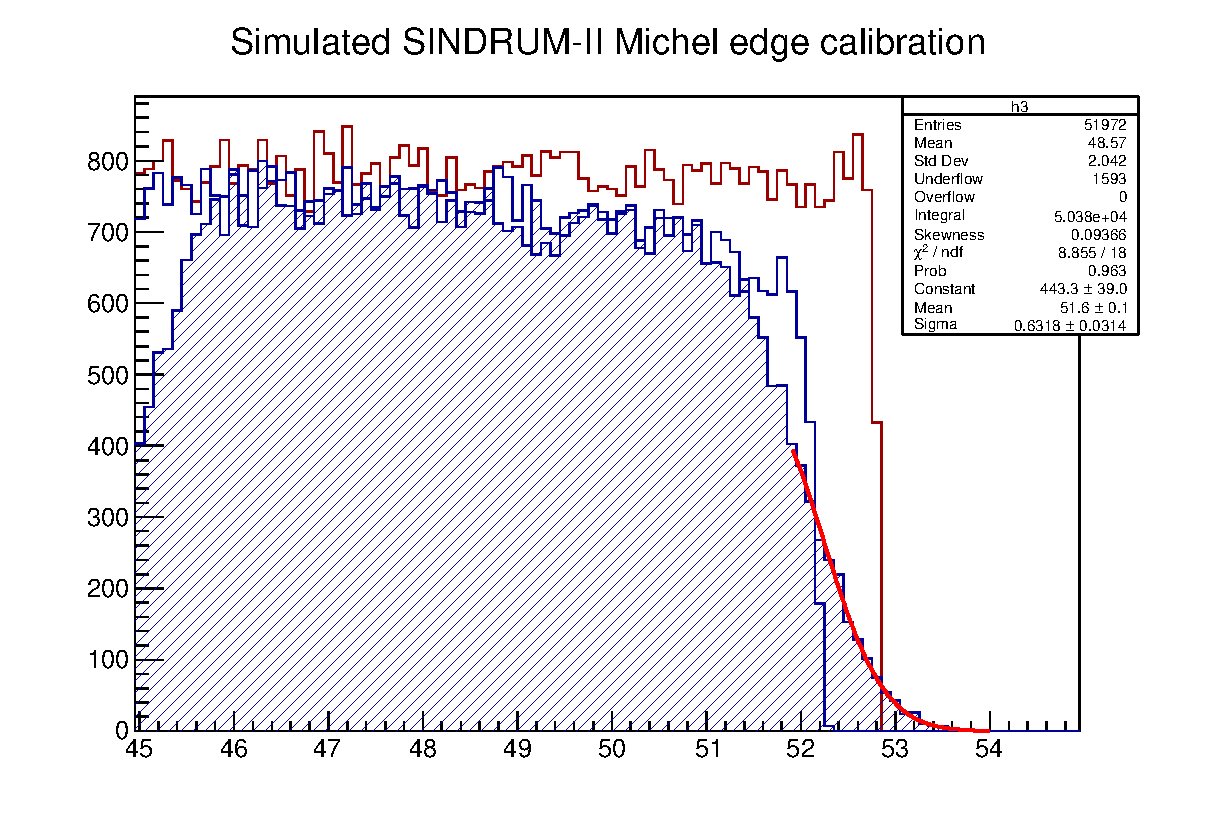
\includegraphics[width=0.99\textwidth]{figures/pdf/simulated_sindrum_ii_michel_calibration}
    }
  };
  % \node [text width=6cm, scale=0.8] at (4.5,6.4) {mu2e-18894 by Kevin Lynch and Jim Popp};
\end{tikzpicture}
% \caption{figure} {
\caption{
  \label{fig:sindrum_ii_michel_calibration}
  A flat spectrum with the right edge at 52.8 MeV is shown in red,
  the same spectrum convolved with the expected SINDRUM-II energy losses is in blue,
  and then this distribution convolved with a Gaussian with $\sigma$ = 0.55 MeV is shaded.
}
% \vspace{0.1in}
\end{figure}

%%%%%%%%%%%%%%%%%%%%%%%%%%%%%%%%%%%%%%%%%%%%%%%%%%%%%%%%%%%%%%%%%%%%%%%%%%%%%% 

%%% Local Variables:
%%% mode: latex
%%% TeX-master: t
%%% End:
